\section{Experimental Results}\label{sec:res}

The evaluation of our algorithm to generate axioms can be divided into four experiments.  The first experiment tests the influence of standard support and proportional one to SIFS. The second experiment compares SIFS with GoldMiner to see their performance when adopting different world assumptions. The third experiment compares SIFS with BelNet\textsuperscript{+} which learns schema knowledge from incomplete KBs. The last experiment shows the usefulness of the generated axioms when detecting logical inconsistencies in DBpedia.

It is noted that, we use SIFS-S and SIFS-P to indicate our system using standard support and that using proportional support separately. SIFS-P can be seen as an implementation of Algorithm \ref{alg:miningAlg}. SIFS-S is actually the implementation of Algorithm \ref{alg:miningAlg} by ignoring the computation of proportional support in line 10 and modifying the threshold and proportional support in lines 11-12 and 18-19 for adapting to the change.

\subsection{SIFS-S vs. SIFS-P}
\begin{table*}[t]
%\renewcommand\arraystretch{2}
\centering
\begin{footnotesize}
\begin{tabular}{|c|c|c|c|c|c|c|c|c|}
\hline
\multirow{2}{1cm}{$t_{conf}$}&\multicolumn{2}{|c|}{Precision-subclass} & \multicolumn{2}{|c|}{Recall-subclass} & \multicolumn{2}{|c|}{Precision-disjoint} & \multicolumn{2}{|c|}{Recall-disjoint}\\
 &SIFS-S&SIFS-P&SIFS-S&SIFS-P&SIFS-S&SIFS-P&SIFS-S&SIFS-P\\
\hline
0.7&0.950&0.950&0.995&0.982&0.912&0.981&0.706&0.712\\
0.8&0.970&0.970&0.983&0.973&0.912&0.982&0.706&0.712\\
0.9&0.990&0.990&0.973&0.961&0.923&0.991&0.700&0.702\\
\hline
\end{tabular}
\end{footnotesize}
\caption{Precision and recall of SIFS-S and SIFS-P with different thresholds}
\label{tab:SIFS-SvsP}
\end{table*}

In this section, we compare SIFS-S with SIFS-P by using different thresholds to filter candidate association rules. Table \ref{tab:SIFS-SvsP} presents precision and recall of both systems to generate subclass axioms and disjointness axioms respectively. This experiment is conducted over DBpedia which is the most challenging KB in our dataset due to its huge number of facts.

From the precision and recall to generate subclass axioms we can observe that, both systems perform similarly. When generating disjointness axioms, SIFS-P performs better than SIFS-S. For example, when $t_{conf}$ is 0.8, the precisions of SIFS-S and SIFS-P are 0.912 and 0.982 respectively and both systems have learned 46,411 and ? disjointness axioms separately. At the same time, the recall of SIFS-P is slightly better than SIFS-S. According to this we know that, although SIFS-P produces less disjointness axioms, more correct axioms are contained.

The reason why SIFS-S could find more disjointness axioms but obtain lower precision and recall is that, SIFS-S always omits the big difference between the number of instances of the concepts in a candidate rule (or axiom). Take the disjointness axiom $\textsf{Person} \sqsubseteq \neg \textsf{Chef}$ as an example.
%
When using absolute support, the confidence of the axiom is 0.92. In DBpedia, $\textsf{Person}$ contains 649,644 instances and $\textsf{Chef}$ just contains 470 instances. This huge difference causes the fact that 517,672 instances of \textsf{Person} are regarded as the negative examples of \textsf{Chef}. In this way, very high confidences could be reached for such false disjointness axioms. If proportional support is used, the confidence of the axiom is 0.5. Obviously, the propositional support could improve the quality of the learned disjointness axioms. In the following experiments, we only compare SIFS-P with other systems.

\subsection{SIFS-P vs. GoldMiner}
In this section, we compare the systems SIFS-P and GoldMiner. Both systems adopt association rule mining to generate axioms while the difference is the fact that they use different world assumptions to generate negative examples. The precision and recall of the systems to generate subclass and disjointness axioms can be seen in Figure  \ref{fig:precision-recall-subc} and Figure \ref{fig:precision-recall-disj} respectively. In these figures, 0.7, 0.8 and 0.9 in the horizontal axis indicate the thresholds to filter those rules with lower confidences.

When mining subclass axioms, both systems have achieved very high precisions because almost all subclass axioms generated by them are correct. With respect to recall, SIFS-P performs better in most cases since more subclass axioms have been found by SIFS-P. This reflects the advantage of using type inference. That is, more type assertions recommended by type inference can increase the support of a rule and thus more correct subclass axioms could be generated. Besides, comparing with the precision and recall of systems to generate disjointness axioms, those to generate subclass axioms are higher, especially with respect to recall (see the left figures in Figure \ref{fig:precision-recall-subc} and  \ref{fig:precision-recall-disj}). This has shown that generating disjointness axioms is much more challenging than generating subclass axioms. 

\begin{figure*}
  \centering
  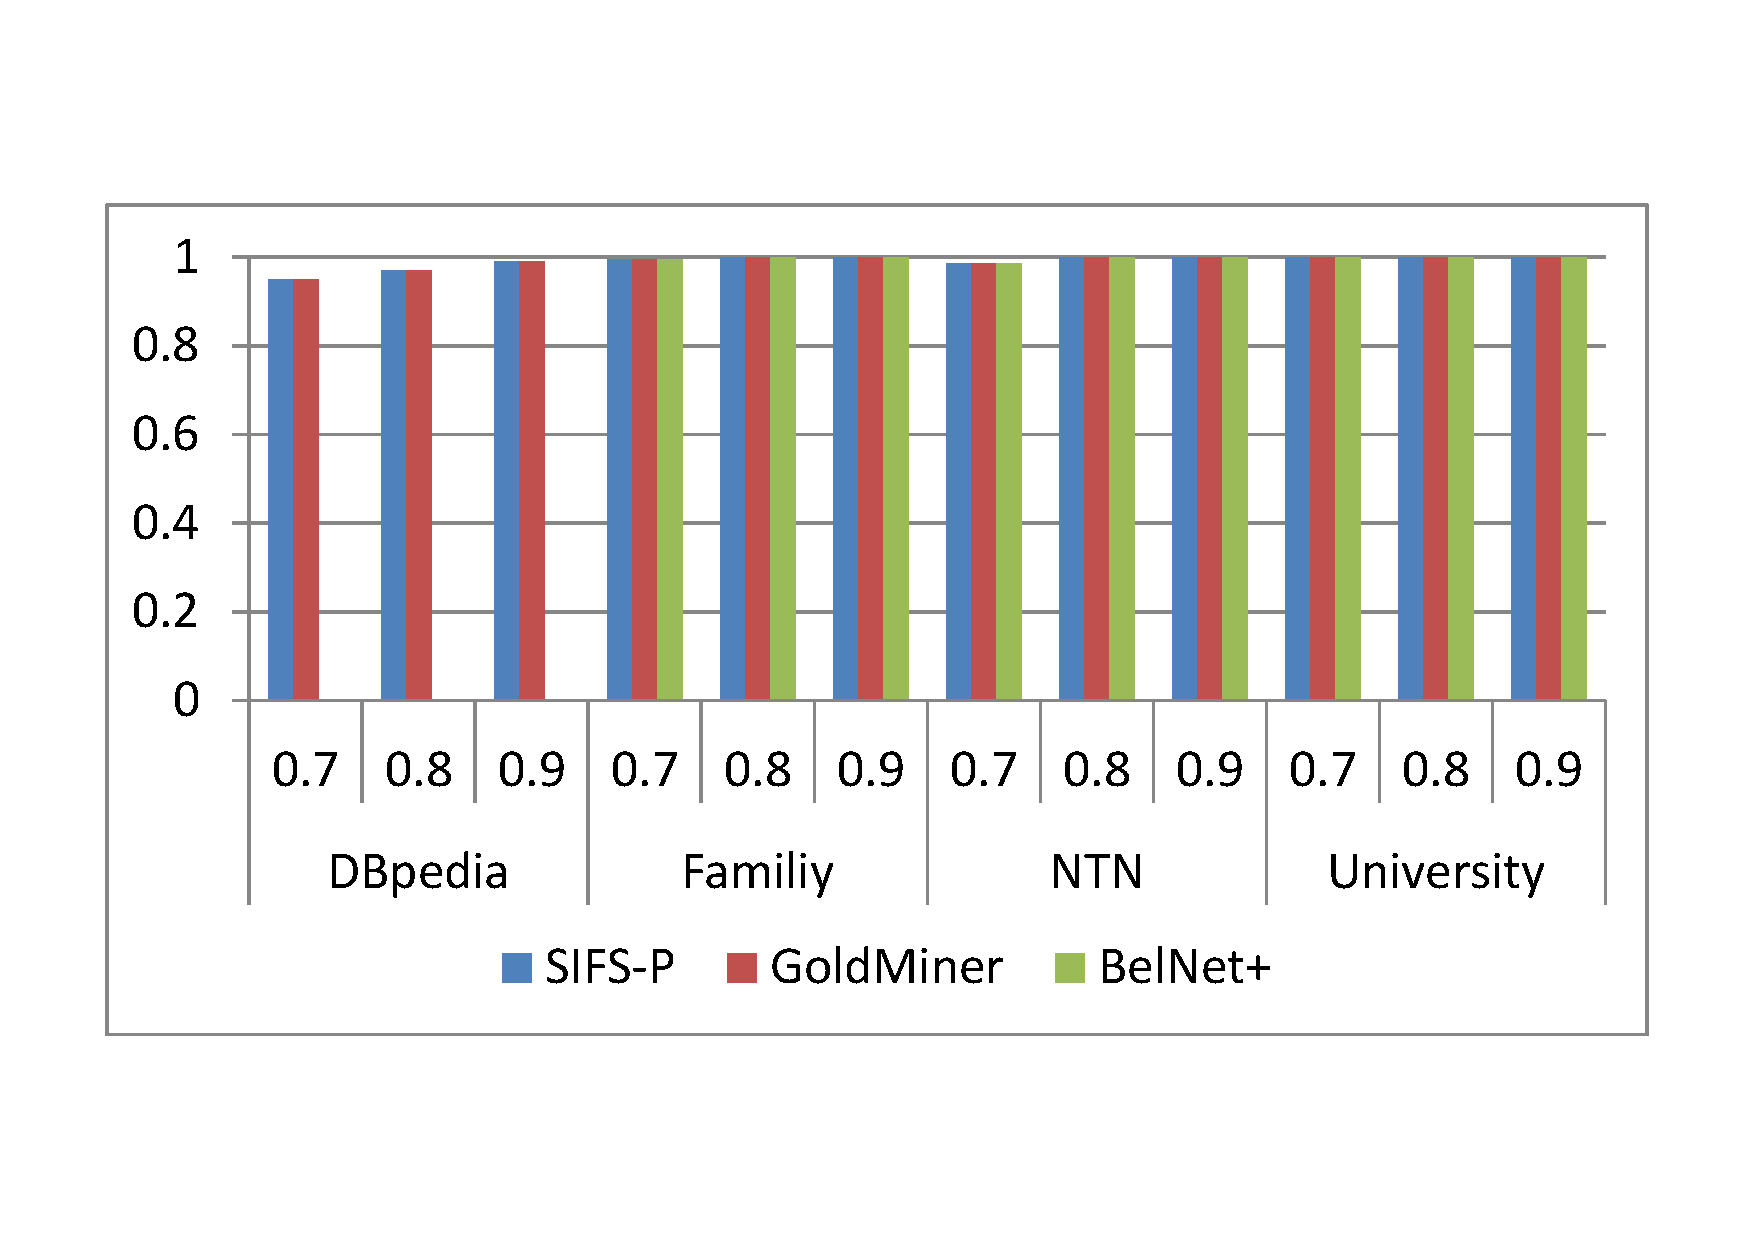
\includegraphics[width=0.49\textwidth]{figs/precision-subc.pdf}
  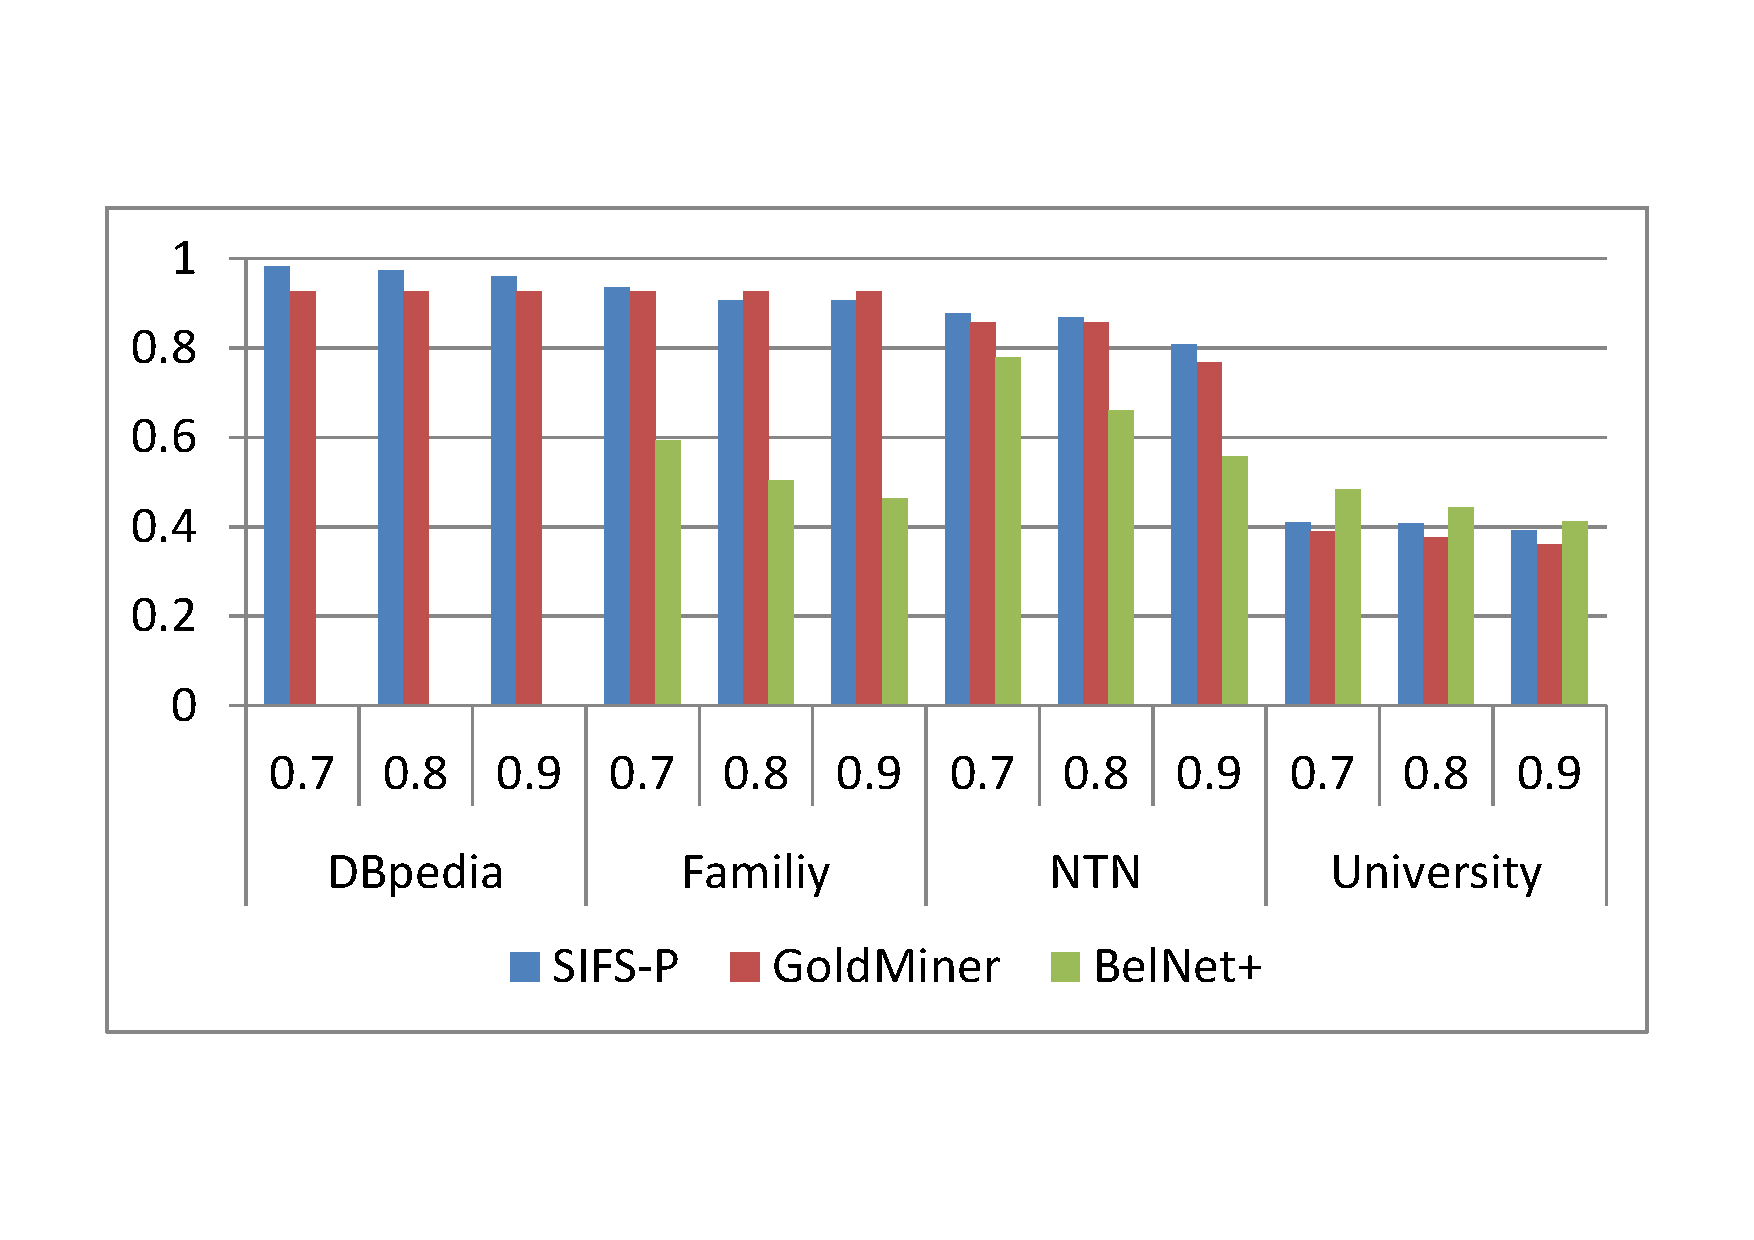
\includegraphics[width=0.49\textwidth]{figs/recall-subc.pdf}
  \caption{Precision (left) and recall (right) of systems to generate subclass axioms}\label{fig:precision-recall-subc}
\end{figure*}
\begin{figure*}
  \centering
  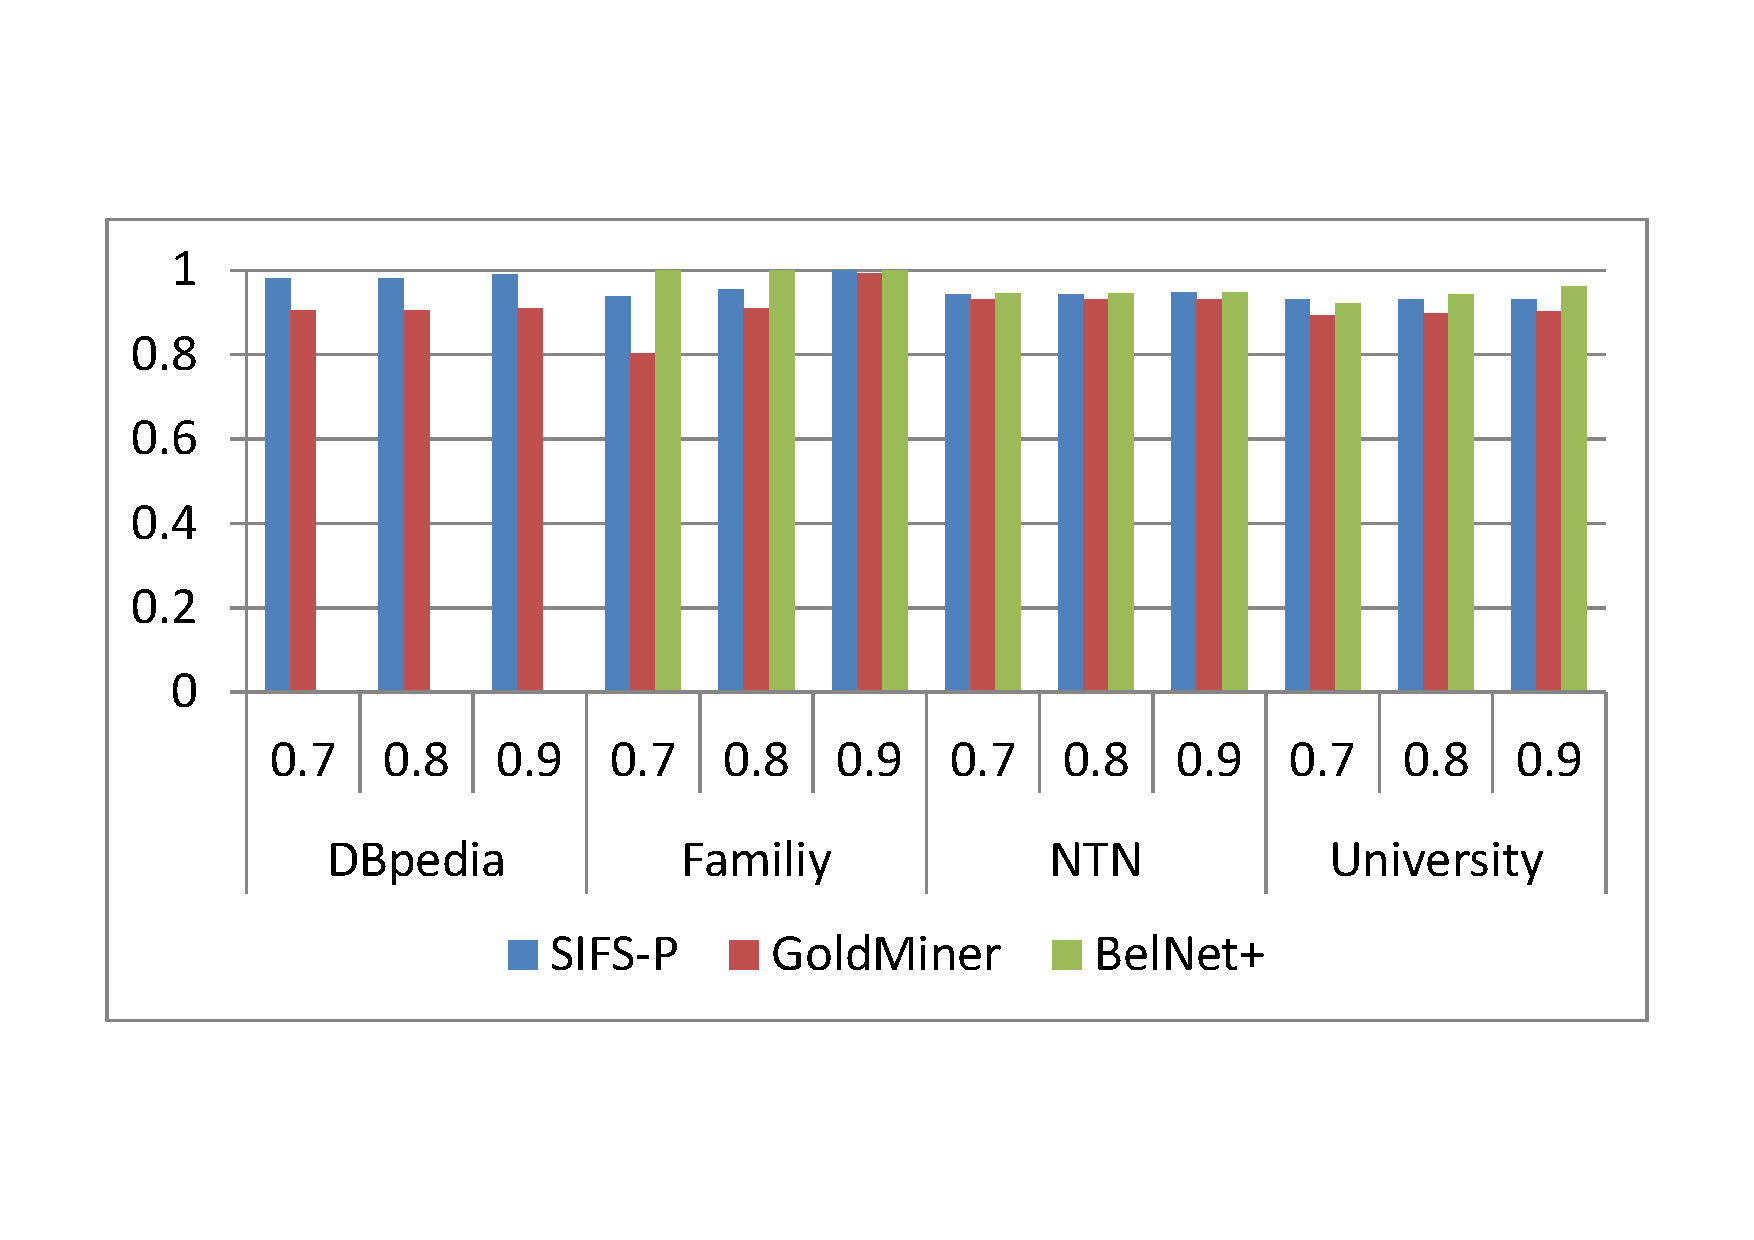
\includegraphics[width=0.49\textwidth]{figs/precision-disj.pdf}
  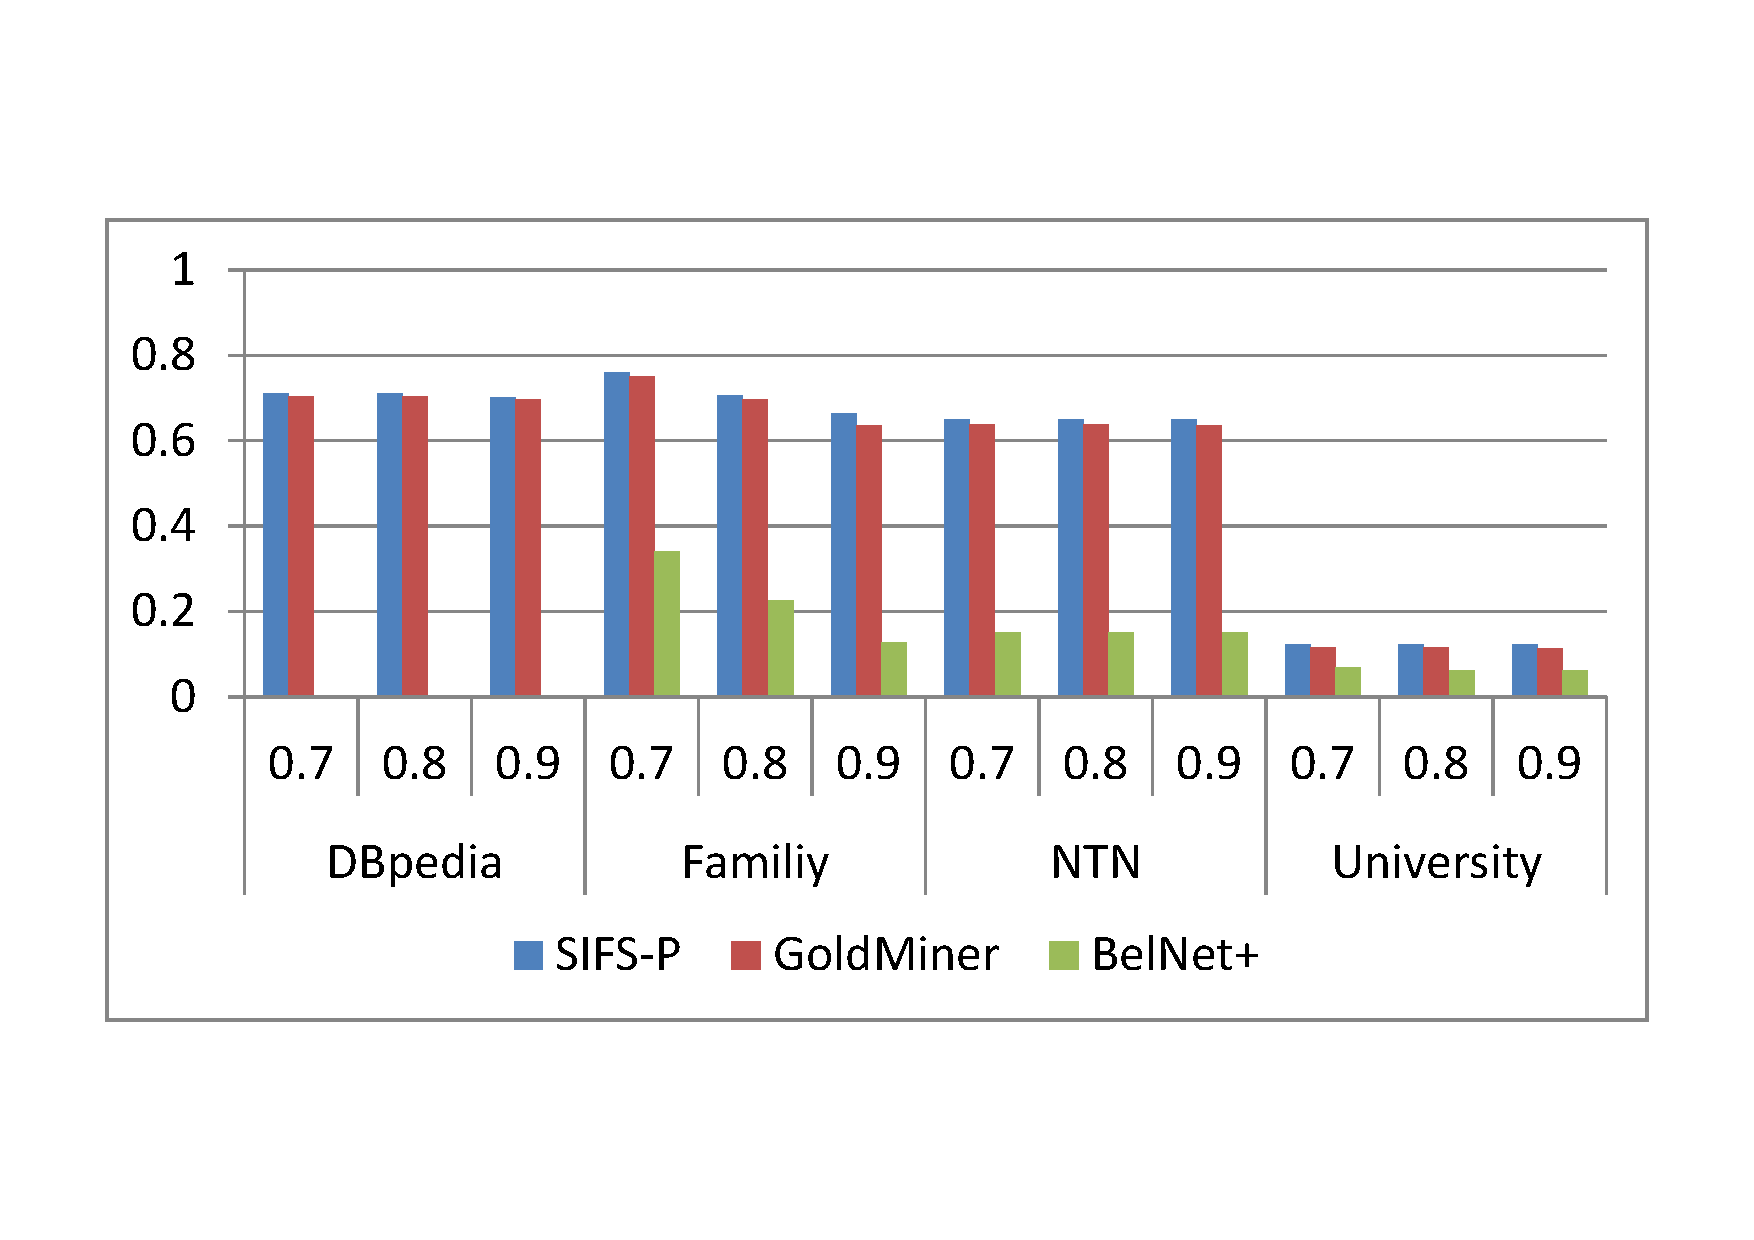
\includegraphics[width=0.49\textwidth]{figs/recall-disj.pdf}
  \caption{Precision (left) and recall (right) of systems to generate disjointness axioms}\label{fig:precision-recall-disj}
\end{figure*}

When mining disjointness axioms, the advantage of using type inference becomes more obvious, especially for DBpedia. When the recalls of SIFS-P and GoldMiner are quite similar, the precisions of SIFS-P are much better. From the right figure of Figure \ref{fig:precision-recall-disj} we can observe that, the difference between the precisions of both systems at any threshold is about 0.1. We summarize some problems to illustrate experimental results.

\textbf{Problem 1.} Negative examples based on CWA will introduce noisy. Because of this, some incorrect disjointness axioms are learned. For example, the confidence of  $WebSite \rightarrow \neg Work$ was 1, that meant there was no common instance in concept $WebSite$ and $Work$

However, in the TBox of DBpedia, the concept $WebSite$ was a subclass of \emph{Work}. In DBpedia, ${Website}$ have 1,852 instances. However, all these instances were not explicitly stated to be the instances of $Work$. Under CWA, each instance of $Website$ was a negative example of $Work$. Therefore, $WebSite \sqsubseteq \neg Work$ was learned by GoldMiner.

\textbf{Problem 2.}  GoldMiner used the standard support. Thus, the standard support learned two competing axioms.

In the subsection 3.4, we will discuss the problem in detail. Our approach, in contrast, will overcome the above problems.
\begin{figure*}
  \centering
  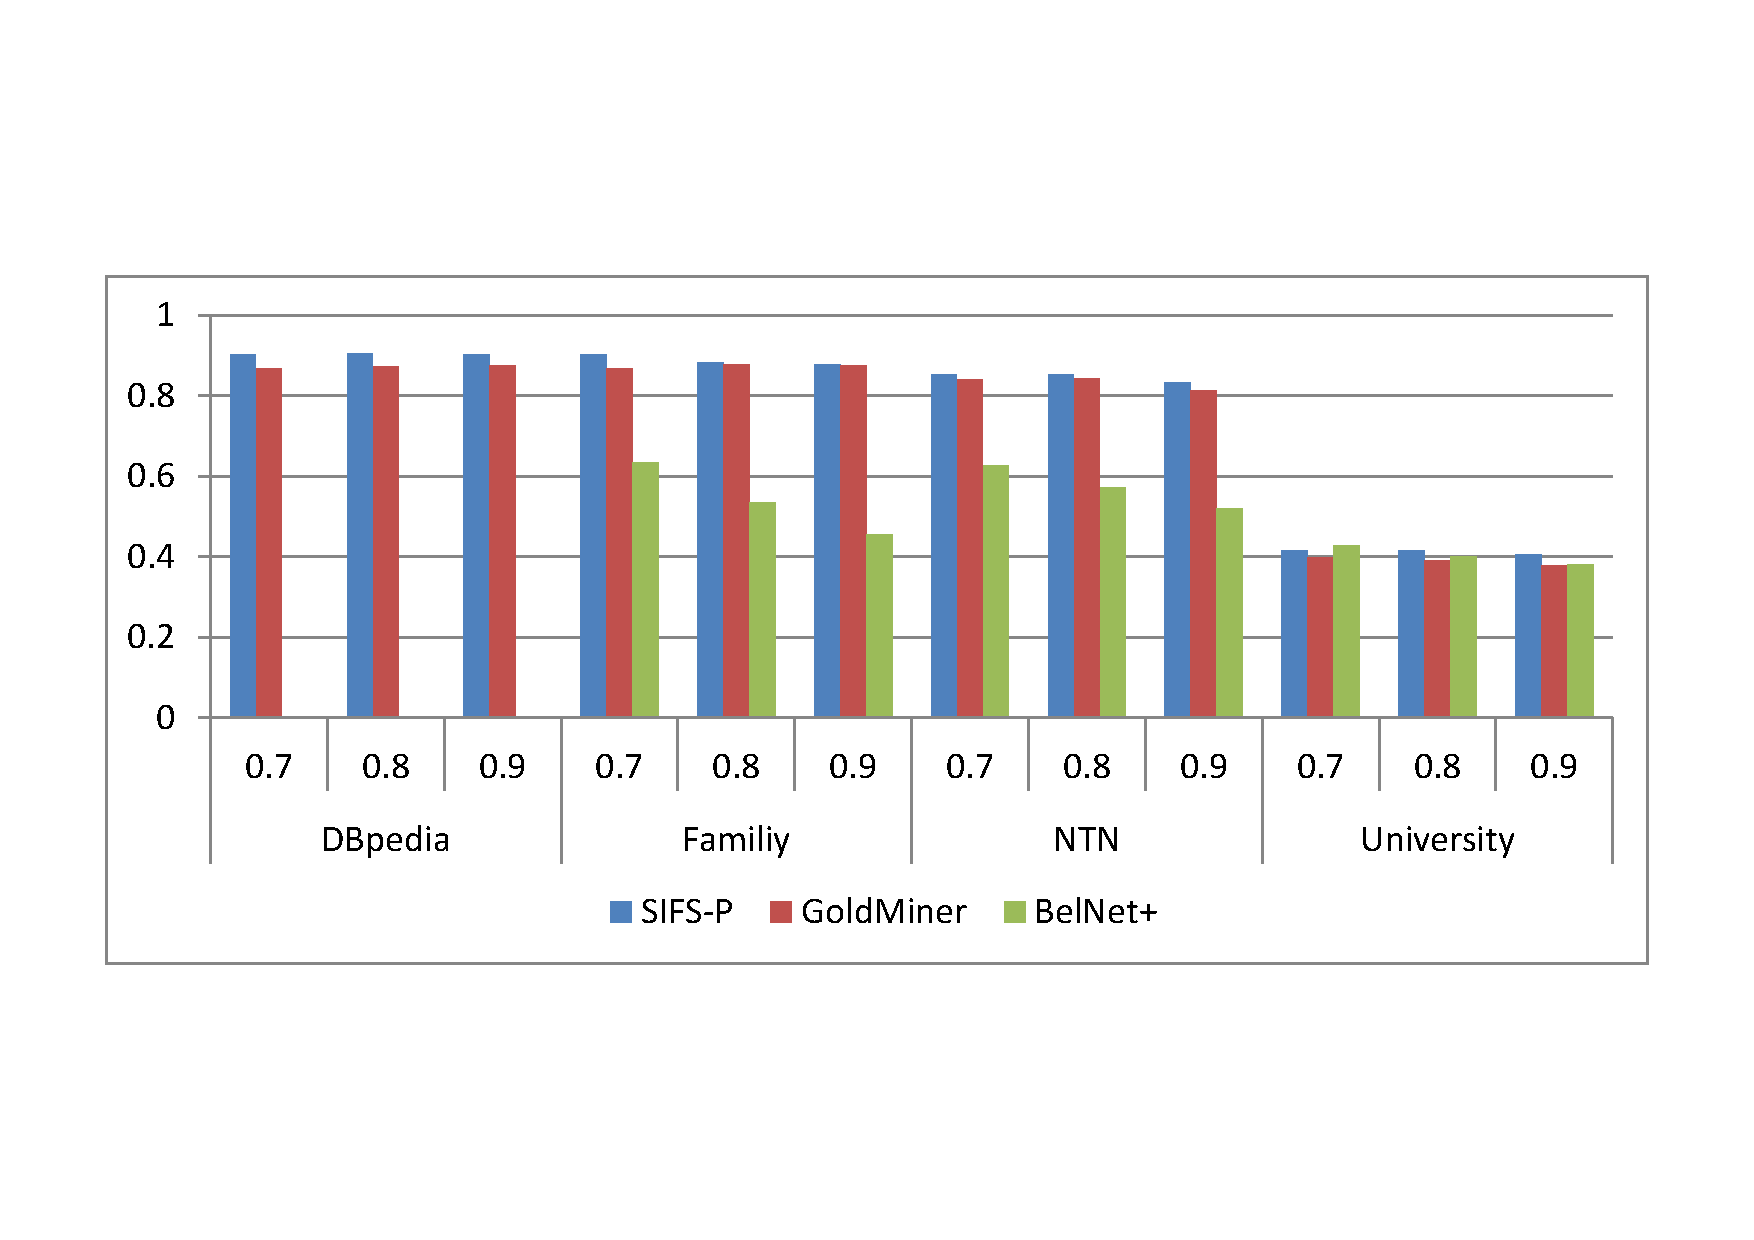
\includegraphics[width=0.75\textwidth]{figs/f1-both.pdf}
  \caption{F1-measure to generate both subclass axioms and disjointness axioms}\label{fig:f1-both}
\end{figure*}

For problem 1, SIFS use a type inference algorithm to generate negative examples. There are two advantages by using SIFS. The first is SIFS supplements the original KB. Supplementing TPs increasing the support of a rule that was filter by GoldMiner. The second is quality of noisy negative examples that are generated by the type inference algorithm is better than using missing TAs as negative examples. After the type inference algorithm is used, some TAs of $Website$ owned had very high probability of instances of \emph{Work}. Thus, SIFS inferred that the concept $WebSite$ and $Work$ were not disjoint but $WebSite$ is a subclass of $Work$ . We resolved the problem 2 by the proportional support. Figure \ref{fig:precision-sub} and Figure \ref{fig:Precision} demonstrated that SIFS outperformed the GoldMiner. According to Figure \ref{fig:Precision} (A) and Figure \ref{fig:Recall} (A), both precision and recall of SIFS were greater than those of GoldMiner.

\subsection{SIFS-P vs. BelNet\textsuperscript{+}}
In this section, we compared SIFS with BelNet\textsuperscript{+}\cite{BelNet+} which focuses on learning TBox from an incomplete ABox. The goal of BelNet\textsuperscript{+} is very similar to SIFS. It transfers the TBox learning into the inference in the extension of Bayesian Description Logic Network. The structure of the BelNet\textsuperscript{+} is leveraged to evaluate relations between the two concepts. We compared performances of BelNet\textsuperscript{+} with that of SIFS. 

In BelNet\textsuperscript{+}, The precision of all KBs was more than 0.9. However, BelNet\textsuperscript{+} only can learn tens of or hundreds of disjointness axioms. Thus, the recall of BelNet\textsuperscript{+} was not good. BelNet\textsuperscript{+} depends on the joint probability to learn the disjointness axioms. In the training stage, the number of instances belonging to the pair of concepts was not large enough, which caused that a lot of disjointness axioms discarded in the stage of constructing the network. The experimental results showed that SIFS can learn more disjointness axioms because more instances can be inferred. The precision of SIFS approximates to BelNet\textsuperscript{+}, but the recall of SIFS is higher than BelNet\textsuperscript{+}.



\subsection{Application to Detect Inconsistencies}
In this section, the experiment is conducted to verify the usefulness of our algorithm for detecting logical inconsistencies in DBpedia. For each learned disjointness axiom of the form $C_{i}\sqsubseteq \neg C_{j}$, we use a SPARQL query to retrieve all instances that belong to both $C_{i}$ and $C_{j}$.

Table \ref{tab:inconsitencies} presents the experimental result of detected inconsistencies. From the table we can see that, many logical inconsistencies have been found in DBpedia 3.5.1 by our algorithm. In particular, 99 pairs of disjoint concepts share only 1 to 9 common instances and 4 pairs of disjoint concepts share no less than 10 but less than 50 instances. For example, we can find two type assertions $\textsf{Person(Nuri)}$ and $\textsf{Place(Nuri)}$ from DBpedia. They state that $\textsf{Nuri}$ is an instance of both concept $\textsf{Person}$ and $\textsf{Place}$ which are obviously mutually disjoint. Thus, a logical inconsistency is caused. Before learning disjointness axioms, such inconsistencies cannot be detected due to the incompleteness of schema information.
\begin{table}[t]
%\renewcommand\arraystretch{2}
\centering
\begin{footnotesize}
\begin{tabular}{|c|c|}
\hline
Number of common instances & Pairs of disjoint concepts\\\hline
[1 - 10) & 99 \\\hline
[10 - 50) & 4 \\\hline
[50 - 100)& 0 \\\hline
[100 - 1000) & 0 \\\hline
[1000 - $\infty$) & 0 \\\hline
\end{tabular}
\end{footnotesize}
\caption{The statistics of the inconsistencies}\label{tab:inconsitencies}
\end{table}

\subsection{Conclusion of Experimental Results}

We reported 3 groups of experiments to compare SIFS with different approaches of learning disjointness axioms. We find that:
\begin{itemize}
\item[-] The negative examples that are found by the type inference algorithm are better than the negative examples that are found by CWA.
\item[-] The proportional support can overcome the imbalance problem and can avoid generating the false disjointness axioms.
\item[-] Our approach outperforms the current approaches. High-quality disjointness axioms can help the reasoner automatically find more contradictions in KBs.
\end{itemize}